% Created 2018-08-03 Fri 23:01
% Intended LaTeX compiler: pdflatex
\documentclass[11pt]{article}
\usepackage{graphicx}
\usepackage{grffile}
\usepackage{longtable}
\usepackage{wrapfig}
\usepackage{rotating}
\usepackage[normalem]{ulem}
\usepackage{amsmath}
\usepackage{textcomp}
\usepackage{amssymb}
\usepackage{capt-of}
\usepackage{hyperref}
\usepackage{fontspec}
\setmainfont[BoldFont={Gentium Basic Bold}, ItalicFont={Gentium Basic Italic}]{Gentium Plus}
\usepackage{csquotes}
\MakeOuterQuote{"}
\usepackage{hanging}
\usepackage{polyglossia}
\setmainlanguage{english}
\setotherlanguage{hebrew}
\newfontfamily\hebrewfont{SBL Hebrew}
\usepackage[margin=0.8in]{geometry}
\pagenumbering{gobble}
\author{Steven Tammen}
\date{}
\title{Teaching the Ancients to Type: Better Unicode Text Entry for Ancient Greek}
\hypersetup{
 pdfauthor={Steven Tammen},
 pdftitle={Teaching the Ancients to Type: Better Unicode Text Entry for Ancient Greek},
 pdfkeywords={},
 pdfsubject={},
 pdfcreator={Emacs 25.3.1 (Org mode 9.1.13)}, 
 pdflang={English}}
\begin{document}

\maketitle
\bigskip
\bigskip
\bigskip
\bigskip
\bigskip
\begin{center}
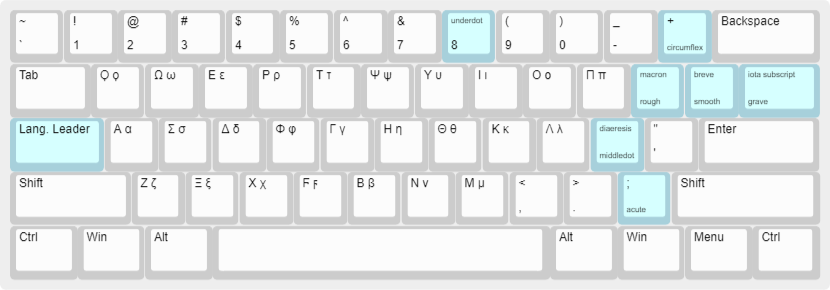
\includegraphics[width=.9\linewidth]{./images/greek-layer.png}
\end{center}

\newpage
\noindent \textbf{Acknowledgements} \\

\noindent This project would not have been possible without the support of the University of Georgia's Center for Undergraduate Research Opportunities (CURO), and the support of my research mentor, Dr. Benjamin M. Wolkow. \\

\noindent I would also like to thank all of the Greek faculty and students that completed this project's research survey. The data from this survey was useful in guiding this project's progression, and also in motivating its completion. Other people care! Hooray! \\

\noindent Finally, I wish to thank my family for all their support and encouragement. I have no doubt talked about keyboards and keyboard layouts enough over the years to drive any group of normal individuals over the edge. But they put up with me nonetheless.

\newpage
\setcounter{tocdepth}{2}
\tableofcontents

\newpage
\pagenumbering{arabic}

\section{About this project}
\label{sec:org87caff2}

\subsection{What is this project?}
\label{sec:org242a507}

While this project has many different goals and subgoals (and continues to add more as additional matters of convenience and usability come up), the essential aim is to create an easy-to-use keyboard layout for ancient Greek while simultaneously creating a framework that can be used to enable efficient entry of non-native languages in general.

Typists for a particular language can usually be classified rather easily into native speakers and non-native speakers. Native speakers type their language "a lot" -- with respect to both frequency and quantity -- while non-native speakers do not. For example, someone who is bilingual in English and Spanish might type approximately 50\% of their text in either language; they have two native languages. However, someone who types 90\% of their text in English and 10\% in German (perhaps to communicate with a colleague or business associate) has only one native language -- English. The lines can get blurry, of course, but the general idea is that one can usually cleanly categorize languages based on how often and how long they are typed: some are typed often and for a long time (native languages), and others are not (non-native languages).\footnote{This is admittedly not exactly how native and non-native languages are typically defined, but hopefully it is a forgivable simplification. People who type a language they did not grow up speaking as a significant percentage of their total volume may not be "native speakers" by some people's definitions, but the terminology is employed here for the purpose of avoiding such verbose titles as "effectively native languages" and "non-effectively native languages."}

In theory, keyboard layouts for native languages should be designed according to certain keyboard design metrics that make typing more efficient. Nowadays, optimization is accomplished through computer programs that change letters in a configuration until additional changes do not improve the layout any more.\footnote{People interested in this process are encouraged to visit \url{http://www.adnw.de}. This site contains much background on the history of keyboard layout optimization, and a well-documented C++ optimizer. The main focus of the site is German layouts, but there is a fair bit of discussion for English layouts as well.} Such an approach is known as a \emph{genetic algorithm}. Examples of this approach may be seen for Chinese in Choe and Liao (2013)\footnote{Choe, Pilsung, and Chen Liao. "Chinese Keyboard Layout Design Based on Polyphone Disambiguation and a Genetic Algorithm." \emph{International Journal of Human–Computer Interaction} 29:6 (2013): 391-403.} and for Arabic in Abandah \emph{et al.} (2008)\footnote{Abandah, Gheith A., Tareq M. Malas, and Sinan Taifour. "Toward Optimal Arabic Keyboard Layout Using Genetic Algorithm." \emph{Proceedings of the 9th Int’l Middle Eastern Simulation Multiconference} (MESM 2008): 50-54.}

Layouts designed in this manner perform better with respect to typing metrics such as low overall hand movement (which helps reduce unnecessary movement away from the home row) and high hand alternation (which helps prevent many characters from getting typed contiguously by one hand while the other sits idle).\footnote{See \hyperref[sec:org02f3267]{§2.2.1} for a thorough discussion of these metrics.} However, since different languages have different frequently used phonetic patterns/letter combinations, so-called "optimal" layouts for different native languages will place even phonetically and orthographically identical letters in very different places.

The question of whether or not it is better for multilingual individuals to try and learn one keyboard layout that is a compromise between their multiple languages or separate keyboard layouts for each language is a fascinating one, but it is ultimately separate from the matters with which this project concerns itself. This project is instead focused on situations of language imbalance -- given that there is a single dominant keyboard layout (presumably for one's native language), what is the best way to type non-native languages?

\subsection{Why this project?}
\label{sec:org58d5fba}

Multilingual text input for non-native languages is a solved problem. By this I mean that at the time of writing, it is possible with various existing software options to enter text both in a primary language and in multiple alternate scripts (e.g., Greek, Hebrew, Cyrillic, Arabic, Devanagari) with relative ease. Thus, it is fair to ask why another project that deals with these things is being undertaken.

While more specific reasons for this project's existence will be addressed below, it is instructive to see some hard data. A survey of Greek scholars and students taken at the outset of this project (N = 184) reveals that while many people are satisfied with current options for typing Greek, many others in turn are not.\footnote{A complete summary of the survey and its results may be found in \hyperref[sec:orgf2463e8]{§5.1}.}

\begin{center}
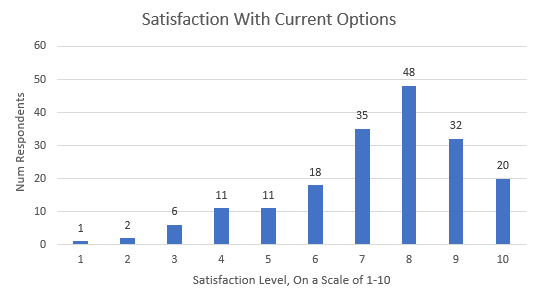
\includegraphics[width=.9\linewidth]{./images/satisfaction.PNG}
\end{center}

If we take satisfaction ratings of 7 or above as "generally satisfied" and 6 or below as "generally unsatisfied," then 49 out of the 184 respondents (26.6\%) are generally unsatisfied with current options. While not overwhelmingly negative, this is not the sort of response one would expect if there were not room for improvement.

\subsubsection{To combat the lack of open source, \emph{customizable} software}
\label{sec:orgdfe1aa8}

This section will use the present state of Greek text input to illustrate how customizable software is currently lacking. \\

\noindent \textbf{Current options for Greek text input} \\

The survey mentioned above contained questions about program usage in an attempt to get an idea of what tools Greek scholars/students generally use to type Greek.

\begin{center}
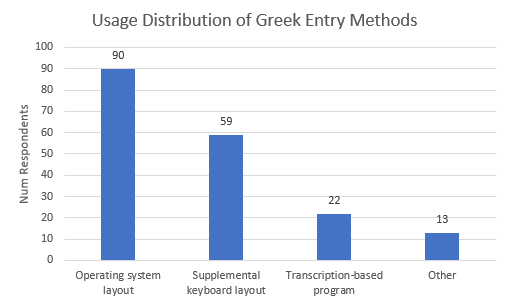
\includegraphics[width=.9\linewidth]{./images/entry-methods.PNG}
\end{center}

\begin{center}
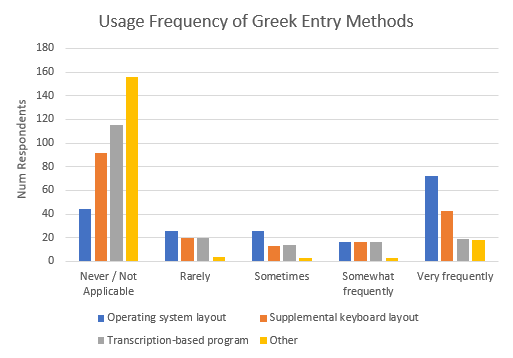
\includegraphics[width=.9\linewidth]{./images/entry-method-usage-distribution.PNG}
\end{center}

Most people either use a default operating system layout (e.g., Windows 10's Polytonic Greek layout) or a keyboard program that gives access to system-wide keyboard layouts (e.g., GreekKeys\footnote{For the website of this specific keyboard project (and also the websites of the other projects mentioned below), please see the table in \hyperref[sec:orga7293a5]{§6.2}.}). Some people use transcription-based programs that employ something like Betacode to match up English and Greek (e.g., SophoKeys), and some people use something else completely, like multilingual word-processing programs (e.g., Yudit, da Grunk). TypeGreek.com and Antioch were two of the more frequent "other" options on the survey. \\

\noindent \textbf{Positive characteristics of existing options} \\

Among different options one can observe several important design characteristics. Most of the solutions are \emph{homophonic}, meaning that alpha is put on the A key, beta on the B key, and so forth:

\begin{center}
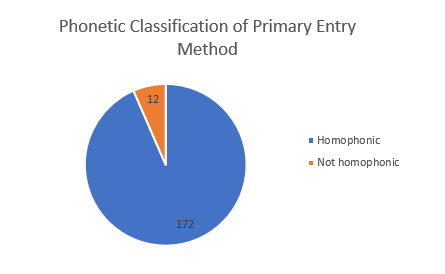
\includegraphics[width=.9\linewidth]{./images/homophonic.PNG}
\end{center}

Some (e.g., da Grunk) attempt to avoid complex chord sequences when entering diacritical marks by using punctuation-based mnemonics, and allow for flexible entry order, meaning that breathing-then-accent or accent-then-breathing (for example) both correctly display. Many (e.g., GreekKeys, SophoKeys) allow for text entry across applications rather than having to copy and paste out of some "special" window. All of these things are definite positives for a typist, especially one switching into Greek text entry from time to time while primarily typing in their native language(s). \\

\noindent \textbf{Customization and open source} \\

However, users who wish to customize things are out of luck with present options. Some people may wish to change how diacritics are handled, for example, or to change which Latin-script letter chi goes on to conform to their preferences (both C and X are popular, but it can be irritating to have to deal with both mappings). Because current options are closed source without significant customization interfaces, this is simply not possible.

Customization and open source software go hand-in-glove, and especially for a program such as this -- which is dealing with a very domain-specific problem that contains much that is subjective and/or related to user preference -- there is significant benefit to making software community-driven. With a community-driven project, different groups of people with different demands can contribute features and functionality separately; the project thus grows to become more than the sum of its parts. Setting up a community-driven environment to create a customizable and open source framework for text entry of non-native languages is the second most important goal of this project (the first being completion of a full Polytonic Greek layer).

Another reason for this project's focus on customizability is the fact that currently available homophonic layouts (at least those that function at the system level) do not work for "nonstandard" keyboard layouts -- they all assume a QWERTY base mapping.

People typing on Dvorak, Colemak, QWERTZ, BÉPO, and so forth may wish to have the benefits of homophonic letter layouts in their non-native languages while retaining their native base layout. For this project, all of the functionality in any language can be implemented on whatever base layout is desired, with full customization as an option; while time constraints mean that only QWERTY will be supported out of the box initially, the underlying structure of the mapping does not rely on QWERTY, and other layouts should be supported in the future.\footnote{Different physical layouts for keyboards will also be supported eventually. Most people type on the standardized ANSI and ISO keyboards, but those who type on things like the Kinesis Advantage or Ergodox -- keyboards that have more keys to work with -- will not have to go through extra steps in customization once the physical configurations are supported.}

\section{Project goals and features}
\label{sec:org5623cd4}

Thus far this paper has examined exactly what this project is interested in at a high level. This section will seek to present a brief summary of this project's main goals and features.

\subsection{Sane defaults combined with ease of use: the principle of least astonishment}
\label{sec:orgd2ef37c}

One notable component of user experience (UX) design is the so-called "principle of least astonishment" (or "rule of least surprise"). \emph{The Art of Unix Programming}, succinctly defines the principle as "In interface design, always do the least surprising thing,"\footnote{Raymond, Eric S. \emph{The Art of Unix Programming}. Boston: Addison-Wesley, 2004. Section 1.6.10, p. 20. Cf. also Section 11.1 "Applying the Rule of Least Surprise," p. 254ff.} and \emph{Principles of Computer System Design: An Introduction} defines it as "The design [of a system] should match the user's experience, expectations, and mental models."\footnote{Saltzer, J. H., and Frans Kaashoek. \emph{Principles of Computer System Design: An Introduction}. Burlington, MA: Morgan Kaufmann, 2009. Section 2.3, p. 85.} In other words, programs should be designed so that they behave consistently (both internally, and with regards to common practices/standards), and do not violate user expectations.

This particular keyboard project does not have a graphical frontend, but does make use of the principle of least astonishment in its design of language layouts and diacritic behavior. The general idea is to create defaults that will make sense to most people, and to structure program behavior around expected patterns of both language use and computer use.

\subsection{Letter placements that make sense}
\label{sec:org80c6834}

Since this project is targeting the typing of non-native languages (see \hyperref[sec:org242a507]{§1.1}), letter placements should be as intuitive as possible for typists that are not typing in a language frequently or for a long time. The survey data gives a good graphical representation of such usage:

\begin{center}
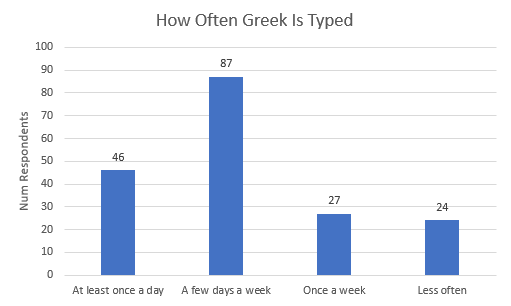
\includegraphics[width=.9\linewidth]{./images/typing-frequency.PNG}
\end{center}

\begin{center}
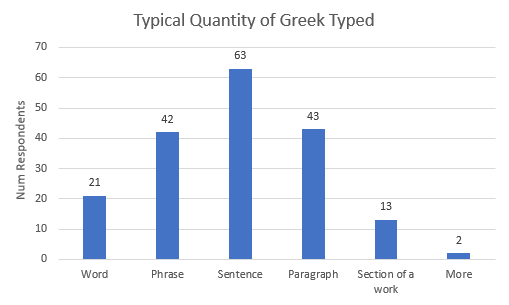
\includegraphics[width=.9\linewidth]{./images/typing-quantity.PNG}
\end{center}

Because long blocks of non-native text are not being typed often, this project makes design decisions that favor memorability over raw optimality.

\subsubsection{Typing performance and keyboard layout considerations}
\label{sec:org02f3267}

Studies of typing have identified some trends in terms of keystroke efficiency and general typing performance. For example, Dhakal \emph{et al.} (2018)\footnote{Dhakal, Vivek, Anna Maria Feit, Per Ola Kristensson, and Antti Oulasvirta. "Observations on Typing from 136 Million Keystrokes." \emph{Proceedings of the 36th ACM Conference on Human Factors in Computing Systems} (CHI 2018): Paper No. 646.}, in a study of 168,000 volunteer typists, found that inter-key intervals (IKIs) -- the time intervals between subsequent key presses, a good predictor of overall typing speed\footnote{Lower IKIs indicate a faster typing speed since IKIs are essentially how much time passes between keypresses; lower IKIs indicate less time between keypresses, and hence a higher overall typing speed.} -- were lower for bigrams (two-letter sequences) that alternated hands (i.e., had one letter typed by one hand, and a following letter typed by the other hand) than for bigrams typed on only one hand. Feit \emph{et al.} (2016)\footnote{Feit, Anna Maria, Antti Oulasvirta, and Daryl Weir. "How We Type: Movement Strategies and Performance in Everyday Typing." \emph{Proceedings of the 2016 CHI Conference on Human Factors in Computing Systems} (CHI 2016): 4262-4273.}, in their overview of previous studies of typing, summarize well-established phenomena and their corresponding measures based on prior studies of professional touch typists; the finding reported above has been noted multiple times in prior studies. Additionally, Feit \emph{et al.} observed that repeated key presses have lower IKIs than same-hand key presses (with keys pressed by different fingers), which in turn have lower IKIs than keypresses that require the same finger to press two different keys in succession.

Dhakal \emph{et. al} also found that faster typists make/need to correct fewer mistakes than slower typists, that faster typists use more fingers on average, and that faster typists have high "rollover percentages" -- a measurement of how many keystrokes begin with other keys already being pressed down from a previous keystroke. Feit \emph{et al.} observed a similar phenomenon in that they came to the conclusion that the preparation of keystrokes leads to lower average IKIs. They also noted that a lower standard deviation in global hand position (i.e., lower overall hand movement from some "home position") similarly leads to lower average IKIs, and that a consistent mapping of finger-to-key ("low entropy")\footnote{What this means is that one and only one finger is responsible for a given key: every time that key is pressed, said finger is used (rather than some other finger). Such a situation eliminates ambiguity (and therefore required mental processing), which is probably why it leads to lower overall IKIs.} has a similar effect.

Pulling these observations together, one arrives at something like the following:

\begin{itemize}
\item Bigrams involving hand alternation are faster (in terms of lower IKIs) than repeated keypresses (i.e., a bigram with only one unique key pressed twice by the same finger), which in turn are faster than (non-same-finger) same-hand bigrams, which in turn are faster than (non-repeated) same-finger bigrams.
\item The ability to "prepare" following keypresses positively associates with typing speed (low IKIs), which helps explain why fast typists have high rollover percentages: mentally lining up future keystrokes makes it easier for fast typists to have multiple keys down at the same time.
\item Low overall hand movement positively associates with typing speed (low IKIs). This is likely mediated through low-movement typists being better able to line up future keypresses.
\item The number of fingers used to type positively associates with typing speed (words per minute: WPM).
\item A low error rate positively associates with typing speed (WPM).
\item A consistent mapping of finger-to-key ("low entropy") positively associates with typing speed (low IKIs).
\end{itemize}

In terms of things that can actually be designed around (it is rather difficult to design a layout that inherently "causes" less errors or a more consistent mapping of finger-to-key), present data supports prioritizing bigram hand alternation, prioritizing low overall hand motion, and minimizing the amount of consecutive non-repeat keypresses involving the same-finger.

\subsubsection{The design of non-native keyboard layouts}
\label{sec:org8eae422}

Given the above discussion, one might wonder if it is worth designing keyboard layouts for non-native language that try to minimize IKIs and maximize WPM by their very design. Once in muscle-memory, they would certainly allow for higher theoretical speeds.

However, the exceedingly great complexity of the cognitive processes behind typing -- see Norman and Rumelhart (1982)\footnote{Norman, Donald, and David E. Rumelhart. "Simulating a Skilled Typist: A Study of Skilled Cognitive-Motor Performance." \emph{Cognitive Science} 6 (1982): 1-36.}, e.g., for a specific proposed model-- makes it difficult to pin down performance causalities, particularly with respect to mental models of keyboard layouts. For example: what effect do semantic groupings of characters have?

As a general rule of thumb, so-called "fully optimized" layouts (which tend to have high hand alternation, low overall hand movement, and low same-finger) will have relatively poor inherent memorability in terms of semantic groups. If someone uses a genetic algorithm to design an optimized layout, it will not keep all the letters in a block or numbers in a row, but mix everything together according to frequency considerations. Humans are very pattern-oriented creatures, and having no apparent structure to characters will inevitably make a keyboard layout more difficult to remember, to some degree. Furthermore, it would seem likely that keyboard layouts that are easier to remember will be easier to get up to speed with, especially if they are not practiced very much.

The issue in all this is that there is not any research that explicitly covers these things,\footnote{At least not any research that I am aware of at the time of writing. It is possible that someone has studied these things in a less formal way, and not published their results.} and certainly not anything specific to ancient Greek. For this reason, it is impossible to say definitely how much easier a semantically-grouped keyboard layout for ancient Greek would be to learn than a fully-optimized keyboard layout, or how much faster people might train it to, say, 35 WPM. The data for this simply does not exist. However, this paper is operating on the assumption that these considerations are non-negligible for most people in most circumstances. The hypothesis coming from such an assumption is this: since people typing non-native languages (including Greek) will not be typing them with great frequency and magnitude, it is more rational to focus on memorability over raw optimization considerations, since layouts that are easier to remember will be faster to learn, and the benefits of "brute forcing" an optimized layout (as one might do for one's native language) will never be realized in typical use cases.\footnote{This does not mean that the discussion in the prior section (\hyperref[sec:org02f3267]{§2.2.1}) is not at all relevant to this project. Raw optimality will be used in a few cases where mnemonics do not work well. See \hyperref[sec:orgd5c000b]{§2.2.4} for more on weighing possible layout methods/procedures within the design.}

It is interesting to note that survey respondents valued both memorability and fast typing highly (see \hyperref[sec:org4dca7a6]{§5.1.12}). As discussed in this present section, these variables are in some sense inversely related if what is meant is theoretical upper bounds on typing speed: layouts that are easy to remember by virtue of mnemonics will not be as efficient as those that totally forgo mnemonics in favor of raw optimality. However, within the realm of actual use, mnemonic layouts may turn out to be faster \emph{in practice} for almost all people -- as this section has argued -- since non-native languages are never typed enough that they become entirely automatic with muscle memory taking over (thereby making memorability less important and raw optimality more important).

\subsubsection{Native-language layouts in muscle memory}
\label{sec:org363ba4a}

The above discussion focused on the interplay of memorability, layout optimality (as measured by hand alternation, overall hand movement, same-finger, etc.), and ease of acquisition in the abstract. However, assuming users of this project can already type on a keyboard layout in their own language (in whatever regard: touch typing, hunting and pecking, etc.), they are not starting from ground-zero: muscle memory already exists.

Let's take the Greek letter omicron. Omicron roughly corresponds in phonetic value to the English letter O; omicron also happens to look like the letter O in both its lowercase and uppercase forms. So, rather than putting omicron on some random key, why not simply place it on the same key as the letter O in English? This would certainly make it easier to remember, since muscle memory for O could be easily applied to omicron.

The trade-offs involved in this decision revolve around whether or not this placement of omicron is optimal given its usage. In Greek, omicron is very frequently followed by upsilon, while the sequence OU is less common in English (although not uncommon in general).  Combining this fact with one of the observations noted in \hyperref[sec:org02f3267]{§2.2.1} -- that sequences of letters typed on the same hand have higher inter-key intervals (i.e., are typed slower) than those that alternate hands -- leads to a question: would it better to forgo the mnemonics of the omicron and O mapping to put omicron on a key more favorable to its usage with upsilon, that is, on a key that was on the hand opposite a mapping of upsilon to U? At least on QWERTY, where O and U are both next to each other on the right hand, there is no way to mnemonically map omicron to O and upsilon to U while having the omicron-upsilon diphthong split up across both hands.

This is a single example -- there are many others that could be adduced for Greek alone, not to mention other non-native languages. Greek and English use letters that look and sound similar (like omicron and O and upsilon and U) differently, so it is no surprise that the typing metrics discussed above might suggest putting corresponding letters in different key locations. But it is difficult to change a few letters without changing the whole layout, and once mnemonics are lost, all these new key locations must be \emph{learned}, and, importantly, kept separate from the locations of look-alike/sound-alike letters in other language layouts (so as not to cause retroactive interference). This is to say, while fully-optimized layouts have undeniable theoretical advantages, they also have opportunity cost since they are not learned in the void (unlike one's first/native language layout).

Given the conclusions of the prior section, all that is being hypothesized is that the opportunity cost introduced by dropping mnemonics always exceeds the hypothetical benefits of optimized layouts for the circumstances under which most people type non-native languages (viz., not frequently, and not for a long time). Because associating a new layout with an old layout lets typists reuse neural pathways that are already in place rather than forming new ones from scratch, it is typically best to associate a keyboard layout for a non-native language with a keyboard layout for a native language already in muscle memory.

\subsubsection{Issues in constructing associations}
\label{sec:orgd5c000b}

If we accept the premise that it is best to form correspondences between non-native languages and keyboard layouts already in use, then it follows that we need some formalized system for doing so.

Layouts derived from phonetic matching are typically called "homophonic layouts." While homophonic layouts are excellent when correspondences exist, there are some letters in Greek that have no clear English equivalent; psi, for example, corresponds to the sound pattern in English that is represented by the two-letter sequence "ps." These must be dealt with separately.

The association (henceforth keymap, short for "key mapping") below for Greek attempts to solve such issues in a systematic way. Following the hypothesis presented above (namely, that memorability is a more important concern in these circumstances than raw optimality), priority is given to phonetic correspondences, then visual correspondences, then transcription correspondences, then, finally, to raw optimality.

The ordering of priority above is not based on any hard data (as no such data exists at present, as above), but based on the principle of least astonishment (see \hyperref[sec:orgd2ef37c]{§2.1}) and logical consistency:

\begin{enumerate}
\item Following the principle of least astonishment, if "most" keys are being placed by phonetic correspondence, it makes sense to use phonetic correspondence as the primary determiner of non-native character position, wherever possible.
\item Following this, visual correspondences are used since they do not depend on any particular system, and also have greater "astonishment factor" for alternate keymaps than transcription correspondences (particularly in the case of Greek, which shares many graphemes with English in lowercase and especially uppercase forms). For example, eta in Greek is almost universally put on the letter H in keyboard layouts, since capital eta \emph{is} the grapheme H.
\item Transcription correspondences come next, in that they are a better mnemonic than nothing. Transcription correspondences work best for letter-based transcription (i.e., transcription that does not involve the used of special diacritics), especially that involving only single graphemes.
\item Finally, raw optimality is used when none of the mnemonics work. The letter theta in Greek, for example, has no phonetic \emph{letter} equivalent in English (even though we use [θ] all the time), has no letter look-alikes, and is commonly transliterated as th or tʰ, which doesn't help create any good associations (since tau makes the most sense for the English letter T). So theta is placed on a key that performs best with respect to the goals of high hand alternation, low overall hand movement, and low same-finger.
\end{enumerate}

\subsection{Greek letter placements}
\label{sec:orga761955}

\subsubsection{Phonetic correspondences}
\label{sec:orgb7bdee0}

Greek is a challenging language to pin down phonetically inasmuch as it has undergone a great deal of change (even if one limits the time of interest from c. 800 BC to c. 200 AD). In later Greek, theta and phi were definitely pronounced as fricatives (as [θ] and [f], respectively); however, in early Attic, they were pronounced as aspirated stops.\footnote{One may read more about these sound changes in W. Sidney Allen's \emph{Vox Graeca: a Guide to the Pronunciation of Classical Greek}.} This project does not pretend to settle the debate of which pronunciations should be used in general, but simply uses [θ] and [f] for the pronunciations of theta and phi because doing so is expedient: eliminating phonetic overlap (from the English perspective) makes a phonetic mapping less ambiguous. Purists will forgive me, I hope.

If a letter has any unambiguous English equivalent (even if it has additional sounds in some contexts not found in English, as with gamma being pronounced as [ŋ] before velars), I have opted to match them. I have also opted to match "near misses" -- sounds that aren't quite identical (or at least are not so on an exact 1:1 level), but are close enough that a native English speaker perceives them as obviously connected (such as rho and R, and many of the vowels).

\begin{center}
\begin{tabular}{lll}
Greek letter & IPA & English match\\
\hline
Α α & [a], [aː] & A\\
Β β & [b] & B\\
Γ γ & [g], [ŋ] (before velars) & G\\
Δ δ & [d] & D\\
Ε ε & [e] & \\
Ζ ζ & [zd] & Z\\
Η η & [ɛː] & \\
Θ θ & [θ] & \\
Ι ι & [i], [iː] & I\\
Κ κ & [k] & \\
Λ λ & [l] & L\\
Μ μ & [m] & M\\
Ν ν & [n] & N\\
Ξ ξ & [ks] & X\\
Ο ο & [o] & \\
Π π & [p] & P\\
Ρ ρ & [r] & R\\
Σ σ & [s] & S\\
Τ τ & [t] & T\\
Υ υ & [y], [yː] & U\\
Φ φ & [f] & F\\
Χ χ & [kʰ] & \\
Ψ ψ & [ps] & \\
Ω ω & [ɔː] & \\
\end{tabular}
\end{center}

This "first pass" at matching gets us pretty far, but there is still some work to do. There are basically two kinds of letters that have not been matched at this point: those that are ambiguous in terms of phonetics (ε/η, κ/χ, and ο/ω), and those that have no single-letter English phonetic equivalent (θ, ψ).

\subsubsection{Visual correspondences}
\label{sec:org1becf19}

Look-alike letters, even if they have no phonetic correspondence, can be an easy way to remember letters. Anything that helps create mental associations can help speed up the learning process. Both uppercase and lowercase forms are considered.

\begin{center}
\begin{tabular}{ll}
Greek letter & English match\\
\hline
Ε ε & E\\
Η η & H\\
Θ θ & \\
Κ κ & K\\
Ο ο & O\\
Χ χ & \\
Ψ ψ & Y\\
Ω ω & w\\
\end{tabular}
\end{center}

Uppercase epsilon, eta, kappa, and omicron look identical to the uppercase English letters E, H, K, and O, respectively (and lowercase omicron also looks identical to  lowercase O). Furthermore, lowercase omega looks very similar to lowercase W. Uppercase psi looks similar enough to uppercase Y that it is worth using as a mnemonic, in my opinion. Note that while chi looks very similar to the English letter X, we are already using X to represent xi. This second round leaves us with only two letters remaining: theta and chi.

\subsubsection{Transcription correspondences}
\label{sec:orgcfbe292}

One of the problems with transcription is that it is not terribly standardized, and where standards exist, they exist in plural. An excellent treatment of Greek transcription/transliteration standards comes from Verbrugghe (1999)\footnote{Verbrugghe, Gerald P. "Transliteration or Transcription of Greek." \emph{The Classical World} 92, no. 6 (1999): 499-511.}, who identifies five main schemes: Latin transcription, Beta Code transliteration, Latin transliteration, Modern Greek transcription, and Modern English transcription. Here are our letters of interest in each of the five schemes:

\begin{center}
\begin{tabular}{llllll}
 & Latin & Beta Code & Latin & Modern Greek & Modern English\\
Greek letter & transcription & transliteration & transliteration & transcription & transcription\\
\hline
Θ θ & th & q & th & th & th\\
Χ χ & ch & x & ch & h & kh\\
\end{tabular}
\end{center}

Of these five schemes, Beta Code transliteration (used, e.g., by TLG and Perseus) and Latin transliteration are not really used in representing Greek text outside of search boxes, at least in the modern day. Modern Greek transcription is not sufficient for transcribing ancient Greek, and so is not of interest for this particular implementation. This leaves us with Latin transcription and Modern English transcription.

As Verbrugghe discusses, Latin transcription has been around in some form since the time of the Romans, and for better or for worse, many English words that have Greek origin are almost universally used in the form of their Latin transcriptions. Modern English transcription, on the other hand, is more concerned with closely mirroring the underlying Greek forms and pronunciation (free from the influence of the Latin language and Roman culture). A prime example of the differences may be observed in the transcription of Ἀχιλλεύς: most English speakers would recognize "Achilles" as the Greek hero of the \emph{Iliad}, but fewer would be able to recognize "Akhilleus," even though it is a much more accurate representation of the underlying Greek.\footnote{Of note is that Richard Lattimore's influential translation of the \emph{Iliad} does in fact use Akhilleus instead of Achilles.}

For our purposes, it is enough to note that ch is a fairly common transcription used of chi. Thus, even though the mnemonics are not perfect, there is some support for placing chi on C.

\subsubsection{Raw optimality}
\label{sec:org34dabb5}

Theta is a tricky letter to place, since no correspondence efforts help with it.\footnote{While Beta Code transliteration does use Q for theta, this is not a helpful mnemonic for anyone who does not use Beta Code regularly, and this mapping does not have the benefit of having Greek words commonly \emph{transcribed} with Q in place of theta. Frequent users of Beta Code may wish to give Q a higher priority than the other letters (J and V) for the placement of theta, but this project does not.} English letters that are left include Q, V, and J; none of these letters is particularly satisfying as a choice, since they are all essentially arbitrary. Because there is no other good basis for assigning theta, an analysis of raw optimality is used.

\hyperref[sec:org02f3267]{§2.2.1} noted that high hand alternation, low overall hand motion, and low same finger are all desirable. While typically judgments involve weighing all three of these factors (and others as well) because it can be hard to tell which locations are better than others, since J is one of the home positions for QWERTY (and V and especially Q require substantially more hand motion), J is a strictly superior placement option. Thus, this project uses J for theta.

\subsubsection{The full Greek letter keymap}
\label{sec:orgf02a408}

Based on the letter choices from the last four sections, one arrives at the following letter keymap, which is the default for this project's Greek layer:

\begin{center}
\begin{tabular}{ll|ll}
Greek letter & Corresponding Key & Greek Letter & Corresponding Key\\
\hline
Α α & A a & Ν ν & N n\\
Β β & B b & Ξ ξ & X x\\
Γ γ & G g & Ο ο & O o\\
Δ δ & D d & Π π & P p\\
Ε ε & E e & Ρ ρ & R r\\
Ζ ζ & Z z & Σ σ & S s\\
Η η & H h & Τ τ & T t\\
Θ θ & J  j & Υ υ & U u\\
Ι ι & I i & Φ φ & F f\\
Κ κ & K k & Χ χ & C c\\
Λ λ & L l & Ψ ψ & Y y\\
Μ μ & M m & Ω ω & W w\\
\end{tabular}
\end{center}

\subsection{Diacritic and punctuation placements that make sense}
\label{sec:org7079960}

Placement of diacritic and punctuation keys is one of the key areas that this project distinguishes itself from others. Many (but not all) keyboard layouts for languages like Greek use either dead-keys or complicated chords (Ctrl + Alt/Option + something) to enter diacritics, which is far harder to remember than a single key equivalence, particularly a key equivalence with visual correspondence. Single keys (even those that require shift to enter) are also much faster to type in general: while it is possible to reduce the IKIs between keypresses to some degree (see \hyperref[sec:org02f3267]{§2.2.1}), an extra keypress will always be an extra keypress (i.e., cause an extra interval between keypresses). Survey respondents overwhelmingly rated the single-key method of entering diacritics as their first choice:

\begin{center}
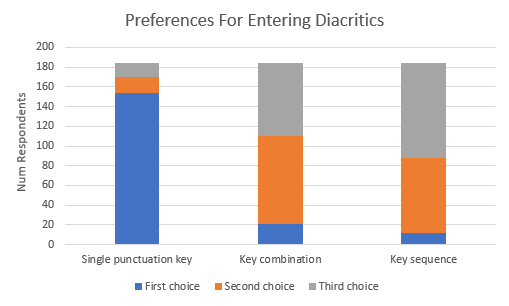
\includegraphics[width=.9\linewidth]{./images/diacritic-entry-preferences.PNG}
\end{center}

Since diacritics don't have phonetic value or any transcription equivalencies most of the time, finding memorable places for them relies comparatively more on visual correspondences and raw optimality. The visual correspondences are a little less obvious as well (e.g., ":" yields a diaeresis as opposed to "a" yields α). However, there is another variable at play here that was not present for letters: semantic correspondences. If different languages use different symbols to indicate questions, exclamations, pauses, and so forth, an obvious mnemonic is matching keys based on similar sentence function. In many ways this is the "phonetic matching of punctuation," inasmuch as keys are being matched directly based on expected usage (i.e., according to the principle of least astonishment).

According to these observations, priority is given to semantic correspondences, then visual correspondences, and then to raw optimality. Note the similarities to the order of priority for letters: in many ways, we are running through the exact same procedure for a different class of characters.

\subsection{Greek diacritic and punctuation placements}
\label{sec:orgf8a2889}

\subsubsection{Establishing available keys}
\label{sec:orgd4aa88d}

Greek has a variety of diacritics that are an essential part of the language. According to our plan of putting these diacritics on English punctuation keys, it is necessary to figure out which punctuation keys are "free" when typing in ancient Greek.

\begin{center}
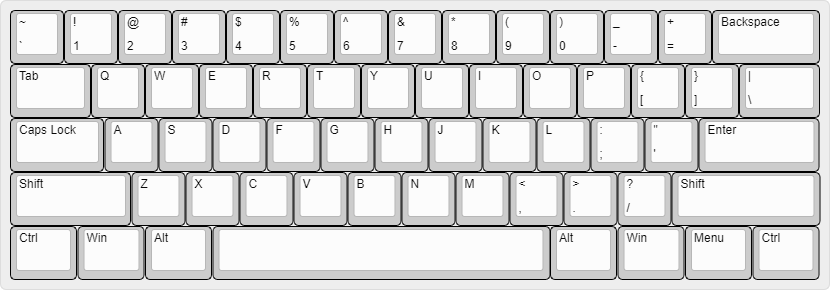
\includegraphics[width=.9\linewidth]{./images/base.png}
\end{center}

This is the ANSI 104 key layout with the function keys and right side of the keyboard (arrow keys, number pad, etc.) removed to save space. This physical layout is very common in the English-speaking world, and will be the one used in all discussions of key placement from here forward.

\begin{center}
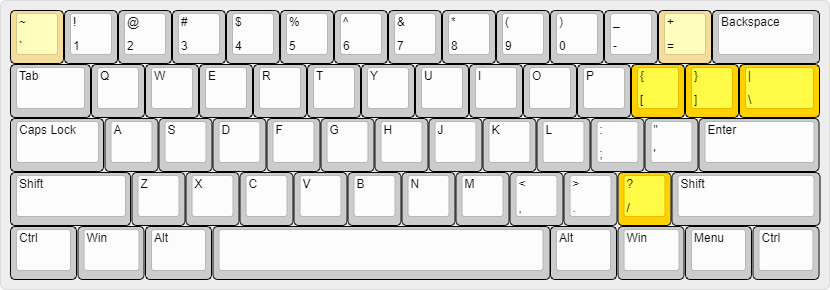
\includegraphics[width=.9\linewidth]{./images/unused-no-shift.png}
\end{center}

This image highlights unused punctuation keys that do not require shift. Numbers are ignored so that they may typed regularly if wished (and to stay consistent across languages). Note that the semicolon is ignored here as well, for the moment, since it is "used" as the Greek question mark. We will return to it later. The apostrophe and hyphen both have uses (as a marker of elision and as an affix marker, respectively), so they have been excluded as well.

The two keys on the number row have been highlighted in a paler color, to indicate their relatively less favorable position. Keys on the number row require a great deal of hand movement to access, which makes them slower to type (see \hyperref[sec:org02f3267]{§2.2.1}). Typing a key on the number row requires moving one's hand up, shifting it out of position for any following keypresses.

\begin{center}
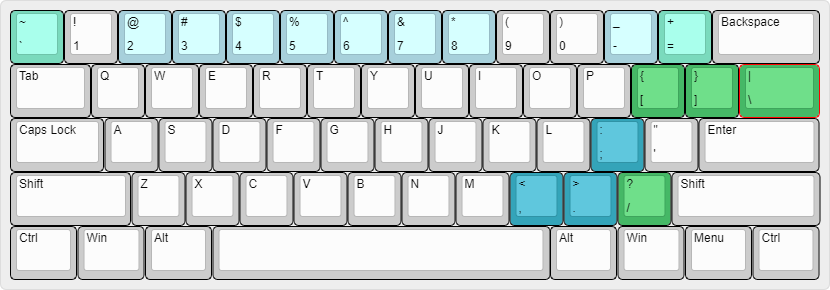
\includegraphics[width=.9\linewidth]{./images/unused-shift.png}
\end{center}

This last image highlights the unused punctuation that do require shift. These keys are strictly inferior to those that do not (i.e., those from the prior picture) since they require a whole additional keypress. Parentheses have been excluded since they are commonly used when writing ancient Greek (even if they do not show up in ancient sources), and the exclamation mark has also been excluded since it is not uncommonly used with imperatives.

Keys that have unused punctuation in both their unshifted and shifted states are shown in green, while those that only have unused punctuation in their shifted state are shown in blue. The shading distinction has been kept: the paler keys on the number row still indicate a relatively less favorable position. All of these keys are options that we can use for our diacritics and punctuation.

\subsubsection{Semantic correspondences}
\label{sec:org4830c94}

Before turning to visual correspondences, it is worth considering direct semantic matches. Greek does not use the English question mark, but it does have a question indicator; similarly, Greek does not use the English semicolon, but it does have a way of indicating a half-stop. It would be very confusing to use different keys for the same meaning, so the Greek equivalents (Greek question mark, Greek middle dot) are placed where their English counterparts are.\footnote{Note that this \emph{is} somewhat confusing in that the semicolon visually represents the Greek question mark, but is mapped to the Greek middle dot since that is the semantic equivalent to the English semicolon. There is not a way to avoid confusion entirely, but semantic correspondences provide the most "intuitive" solution.}

\begin{center}
\begin{tabular}{ll}
Greek Punctuation & Semantic match\\
\hline
Greek Question Mark & ?\\
Greek Middle Dot & ;\\
\end{tabular}
\end{center}

\subsubsection{Visual correspondences}
\label{sec:org546c513}

Most of the diacritic keys can be placed directly using visual correspondences:

\begin{center}
\begin{tabular}{lll}
Grouping & Greek Character & Visual Match\\
\hline
Breathings & Rough & [\\
 & Smooth & ]\\
Accents & Acute & /\\
 & Grave & $\backslash$\\
 & Circumflex & \\
Quantity & Iota Subscript & \(\vert{}\)\\
 & Macron & \\
 & Breve & \\
Other & Diaeresis & :\\
 & Underdot & *\\
\end{tabular}
\end{center}

This leaves us with the macron, breve, and circumflex to place. The circumflex is sometimes represented using a tilde (\textasciitilde{}) shape, but also sometimes represented using an inverted-breve shape. For this reason, this project chooses not to use visual correspondences to match the circumflex: they are ambiguous.

\subsubsection{Raw optimality}
\label{sec:org29cf0cc}

Since the macron and breve are related (they are a pair of quantity-markers with opposite meanings), it would be nice to place them on a pair of keys. That leaves us with either \{ and \}, or with < and >. While all of these keys require shift to access (and so are similar with regards to raw optimality), the former are much more similar to the macron and breve in shape, and are thus used in this layout.

The circumflex is put on = since it does not require shift to access. It could have also been put on the backtick/tilde key (which is essentially the = key's mirror on the other side of the keyboard), but was placed on = to keep all the diacritics on the right side of the keyboard, for consistency.

Note that the visually-chosen keys from the above section also make sense with regards to raw optimality. The most common Greek diacritics (including the breathings and the accents) are all accessible with a single keypress without needing to use shift (which would incur an extra interval between keypresses).

\subsubsection{The full Greek diacritic/punctuation keymap}
\label{sec:org7973a50}

Based on the character choices from the last three sections, one arrives at the following diacritic/punctuation keymap, which is the default for this project's Greek layer:

\begin{center}
\begin{tabular}{lll}
Grouping & Greek Character & Corresponding Key\\
\hline
Breathings & Rough & [\\
 & Smooth & ]\\
Accents & Acute & /\\
 & Grave & $\backslash$\\
 & Circumflex & =\\
Quantity & Iota Subscript & \(\vert{}\)\\
 & Macron & \{\\
 & Breve & \}\\
Punctuation & Greek Question Mark & ?\\
 & Greek Middle Dot & ;\\
Other & Diaeresis & :\\
 & Underdot & *\\
\end{tabular}
\end{center}

This keymap combined with the letter keymap comprises the Greek layout for this project. A basic graphical reference for the layout may be seen below:\footnote{The language leader key is described below, in \hyperref[sec:org3588e31]{§2.7.1}.}

\begin{center}
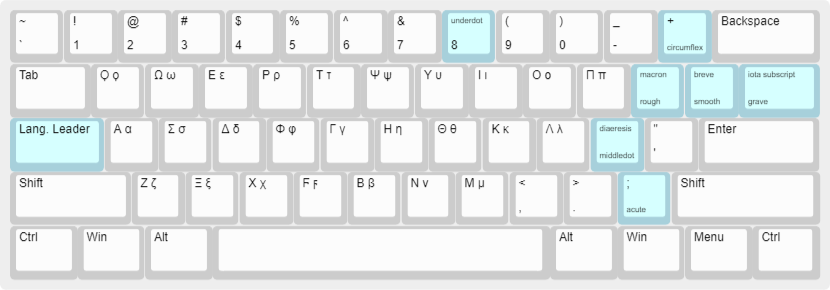
\includegraphics[width=.9\linewidth]{./images/greek-layer.png}
\end{center}

\subsection{Intuitive diacritic and backspacing behavior}
\label{sec:org02ee40c}

Unicode diacritics can be implemented in such a way that adding and removing them becomes complex and messy. For example:

\begin{itemize}
\item If precomposed Unicode is entered with stateless key combinations, adding or removing a diacritic to a letter that has already been typed involves deleting the entire last character and then pressing a new (correct) key combination.
\item If diacritics are entered by means of decomposed Unicode, display problems commonly occur if diacritics are entered in an incorrect order. For example, if a user types alpha then an acute accent, and then, a couple seconds later, decides that that alpha should also have a macron, they typically \emph{cannot} just press the diacritic key for the macron: due to how Unicode treats multiple combining characters, the accent will appear closer to the alpha than the macron, which is typically not the stacking behavior that is desired.
\item If diacritics are entered by means of decomposed Unicode, by default there is no way to change or remove diacritics any way but sequentially. That is, if you have something like alpha + smooth breathing + circumflex + iota subscript, and wish to either remove the smooth breathing or change it to rough breathing, you will have to delete all three diacritics to be able to change the breathing.
\end{itemize}

In this project, diacritics are added to a letter by pressing the \emph{single} keys associated with them, typically linked mnemonically (see \hyperref[sec:org7079960]{§2.4}, above). They can be added in any order, but will always display correctly. They can also be removed in any order: pressing a diacritic key again when the diacritic is already on the preceding letter will remove it, \emph{regardless of the entry order}. Whether it was the last combining character entered or three back, it will be deleted while leaving all the other diacritics untouched. Finally, changing between options within a diacritic category that has mutually exclusive choices does not require deleting an old option before switching to a new option. So, for example, if someone had typed our sequence from above, alpha + smooth breathing + circumflex + iota subscript, but wanted to change that circumflex into an acute accent, all they would need to do is press the diacritic key for the acute accent. The circumflex would get deleted automatically, and replaced with an acute accent. These behaviors align with survey respondents' preferences to immediately see diacritics when typing them, which was generally ranked as the most important design consideration after layout memorability and typing speed:

\begin{center}
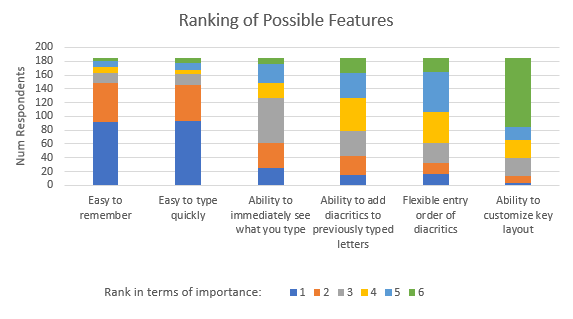
\includegraphics[width=.9\linewidth]{./images/ranking-of-possible-features.PNG}
\end{center}

These behaviors also allow for complete flexibility in entry order, which was another of the options. It was not as important to most people as immediately seeing diacritics as they are typed, but it was ranked as 1st, 2nd, or 3rd important by about a third of respondents -- making it a concern for a significant group. "Smart" diacritic behavior that lets one add and remove diacritics from anywhere in a document was not implemented in the project, despite being one of the more valued features, since it is impossible to implement in a general, program-independent way.\footnote{Programs that let you change diacritics on the fly have some way to access the file/text object you are working on directly (i.e., have read/write permissions for the file on disk and have it open through the kernel, or have some equivalent mechanism on the web). However, such programs are not portable; you cannot go back and dynamically change diacritics if you are typing in an email client, for example, since the text box in the email client is not in the special environment that enables the file checking (lookbehind) necessary for on the fly diacritics.}

Handling individual removal of diacritics in the above manner lets Backspace function exactly how one would expect it to (conforming to the principle of least astonishment): Backspace always deletes one full character -- regardless of the number of diacritics attached to said character -- instead of simply deleting the last diacritic typed.

\subsection{Minimal interference with normal computer use}
\label{sec:org93492a6}

\subsubsection{The language leader key}
\label{sec:org3588e31}

A challenge when dealing with multilingual language input is adding all of the additional functionality (switching between multiple languages, adding Latin-script diacritics for European languages, etc.) without compromising normal computer use in a significant way. Part of the reason for minimizing layout differences is to reduce change friction, but a significant part of it is also to avoid "losing" potential behavior by overriding keys. For example, if someone were to use the Function keys for switching between languages, that person would lose access to the Function keys themselves.

This project minimizes the impact of adding language behavior by encapsulating it all under a single key, henceforth the "language leader key." The language leader key is used to prefix other keypresses to change their behavior. In this way, the only key with changed behavior when typing one's native language is the key assigned to be the language leader key. This project uses CapsLock as the language leader key by default, since most people use it very infrequently and it is in a favorable position. Normal CapsLock behavior is not lost: one simply needs to press CapsLock twice instead of once to access it.

The language leader key is used for three main things: quickly switching between languages using mnemonics (e.g., language leader + g switches to Greek), quickly adding diacritics and special characters for European languages that otherwise do not need a separate layer (e.g., language leader + c adds ç)\footnote{Latin-script language behavior is documented in \hyperref[sec:org805c871]{§5.3}.}, and quickly entering punctuation on non-native layers when it is used for diacritics by default (e.g., ] adds smooth breathing by default for the Greek layer, but a closing bracket may be entered literally with language leader + ]).

\subsubsection{Consistent keyboard shortcuts}
\label{sec:orgadfa384}

Because this project supports normal use of the Control key (and the Alt key, etc.)\footnote{That is, use of the modifier keys with the expected English letters rather than non-native letters.}, users have immediate access to frequent keyboard shortcuts like Ctrl-C, Ctrl-X, Ctrl-V, Ctrl-Z, and so on. Losing these when you are typing in a non-native language can be irritating.

To be fair, it is possible to make keyboard shortcuts work in programs such as Microsoft Word when using an operating system layout. This project does not pretend to be the first that has ever made it easy to keep consistent keyboard shortcuts. However, this project does so out of the box, and does so for all sorts of programs being used (including things like browsers and email clients) rather than just word processors or text editors.

\section{Efficient typing practice and Greek language learning}
\label{sec:org762056f}

Even with the mnemonics described in \hyperref[sec:org5623cd4]{§2}, which make it easier to learn and remember the locations of Greek letters, diacritics, and punctuation, a degree of practice is necessary before the layout can really be used. This section examines what form that practice might take, and how it might be combined with Greek language learning to make more efficient use of time.

\subsection{Repetition in typing}
\label{sec:org9e4a11d}

Within any given language, some words (or parts of words: prefixes, suffixes, etc.) occur with much greater frequency than others. Over time, these words will be typed far more often than words which do not form as essential a part of the language's vocabulary. It follows that if one can learn how to type these words rapidly, their disproportionate occurrence within the language's corpus will lead to significant increases in overall typing proficiency (as measured by speed).

Chua and Liow (2014)\footnote{Chua, Shi Min, and Susan J. Rickard Liow. "The Locus of Word Frequency Effects in Skilled Spelling-to-Dictation." \emph{Quarterly Journal of Experimental Psychology} 67 (2014): 1720-1741.} conducted a study researching why people start spelling high-frequency words faster than low-frequency words. They note that "word frequency effects have been found in spelling-to-dictation with skilled adults such that participants are quicker to initiate spelling of high-frequency words than that of low-frequency words upon hearing the target stimuli." Their study attributes faster first-letter output for high-frequency words to three distinct phenomenon: spoken word recognition, orthographic retrieval, and response execution. Loosely speaking, these can be summarized in order as "figuring out which word, figuring out how to spell it, and figuring out how to translate the spelling into writing/typing movements." For the purposes of this project, it doers not much matter which phenomenon is most important for the faster speeds observed: the general idea is that higher-frequency words are processed faster.

If high frequency words are processed faster, it would make sense for high frequency phrases (sequences of words) to also be processed faster. Bannard and Matthews (2008)\footnote{Bannard, Colin and Danielle Matthews. "Stored Word Sequences in Language Learning The Effect of Familiarity on Children's Repetition of Four-Word Combinations." \emph{Psychological Science} 19 (2008): 241-248.} conducted a study researching frequently occurring "chunks" in child-directed speech, and what effect these stored word sequences have in the speech of children. While their study parameters are markedly different from Chua and Liow's study, the overall significance is similar: frequent sequences are repeated by children more quickly (and accurately) than infrequent sequences. This localizes some of the speed considerations to cognitive processing (i.e., identification of a word rather than lower-level translations of it into hand movements for writing or typing), but doesn't diminish the overall takeaway: it seems that language aspects of human cognition are conditioned by frequency considerations.

These observation are in line with a conception of typing as a form of hierarchical control. Logan and Yamaguchi (2016)\footnote{Logan, Gordon D., and Motonori Yamaguchi. "Pushing Typists Back on the Learning Curve: Memory Chunking in the Hierarchical Control of Skilled Typewriting." \emph{Journal of Experimental Psychology: Learning, Memory, and Cognition} 42 (2016): 1919-1936.} articulate a view of typing in which the translation of language into hand movements is governed by the development of "chunks." In the process of hierarchical control, something in an "outer-loop" of processing is mapped onto several "inner-loop" units (e.g., letters or keystrokes), thus chunking inner-loop units into an outer-loop unit. To use a Greek example, when someone is typing text from a paper source (to quote in research) and comes across the word συμβαίνω, they might first unconsciously split the word into the groups συμ-, βαίν-, and -ω. When typing these, they might further type the root in three units: first β, then αί (a diphthong), and then finally ν. The "loops" present in this example would be the word-level loop (which identifies συμβαίνω as a distinct word), the morpheme-level loop (which identifies the separate morphemes συμ-, βαίν-, and -ω), and the keystroke-level loop. Each loop successively "chunks" lower-level entities into larger blocks that may be cognitively processed as a whole. One might compare this typing-specific process to how a pianist thinks of a chord as "one thing," even though it is composed of many different notes with corresponding finger positions.

According to such a model, learning how to efficiently type is essentially the development of cognitive chunks -- getting to the point where one input unit (e.g., a word) may be translated into a series of motor movements as a whole, without perceptual energy expended to match letters or even keystrokes individually. Repetition underlies the development of these memory chunks. In the study above, the mechanisms for the formation of memory chunks were studied; in all experimental groups, repetition was simply assumed to be necessary. The question then is not whether repetition is necessary for developing efficient typing, but what ought to be repeated so as to form good memory chunks? Based on our working hypothesis, frequent words make the most logical choice.

\subsection{Repetition in learning}
\label{sec:org6428c5a}

In some senses, multiple aspects of language learning involve the building of chunks as well -- in the case of speaking, moving from awareness of distinct phonemes (e.g. letters) to distinct patterns of phonemes (words, phrases), and in the case of reading, moving from awareness of distinct graphemes to distinct patterns of graphemes.\footnote{For an introduction to the cognitive processing present during reading, see Davis, Matt. "Cmabridge." cam.ac.uk. \url{https://www.mrc-cbu.cam.ac.uk/people/matt.davis/cmabridge/} (accessed August 3, 2018).} However, unlike writing, which does not necessarily involve the construction of meaning (e.g., people can easily type words and patterns with which they are unfamiliar), language learning as a whole revolves around not mechanical movements or patterns without specific meaning, but semantic connections. Reading and understanding ancient Greek is a step above being familiar with how the letters are arranged.

With this being said, repetition is by no means useless in language learning. Ansaldo and Ghazi-Saidi (2017)\footnote{Ansaldo, Ana Ines, and Ladan Ghazi-Saidi. "Second Language Word Learning through Repetition and Imitation: Functional Networks as a Function of Learning Phase and Language Distance." \emph{Frontiers in Human Neuroscience} 11 (2017): Paper No. 463.} discuss some of the effects that verbal repetition of non-native words has on the brain at the physical level. In their study, repetition induced neuroplasticity/network integration and led to improvement in behavioral responses both for people whose native language was similar to the non-native language being learned (Spanish and French), and for people whose native language was not similar to the language being learned (Persian and French).\footnote{Another interesting observation of the study is that more distant languages require a higher cognitive load to achieve the same effects. This is not exactly surprising, but it does help explain the difficulty many students have with more "foreign" languages (e.g., those with completely new alphabets and sentence structure) -- even aside from less obvious cognates and shared vocabulary, the languages simply require more from the learner inherently.} This result is in line with prior studies of repetition and vocabulary acquisition.

Repetition in general learning is also well attested to; in particular, so-called "spaced repetition" with delays between exposure has been linked to positive outcomes. Dunlosky \emph{et al.} (2013)\footnote{Dunlosky, John, Elizabeth J. Marsh, Mitchell J. Nathan, Katherine A. Rawson, and Daniel T. Willingham. "Improving Students' Learning with Effective Learning Techniques: Promising Directions from Cognitive and Educational Psychology." \emph{Psychological Science in the Public Interest} 14 (2013): 4-58.} rank "distributed practice" as one of the best learning strategies, and Kang (2016)\footnote{Kang, Sean H. K. "Spaced Repetition Promotes Efficient and Effective Learning: Policy Implications for Instruction." \emph{Policy Insights from the Behavioral and Brain Sciences} 3 (2016): 12-19.} makes a case for spaced repetition with regards to America's lagging academic performance. Given that language learning is a subset of general learning, the benefits of spaced repetition are sure to present in language learning.

Here too it makes sense to focus on frequent words. Major (2008)\footnote{Major, Wilfred E. "It’s Not the Size, It’s the Frequency: The Value of Using a Core Vocabulary in Beginning and Intermediate Greek." Winter 2008.} argues strongly for the study of frequent words in the acquisition of a "core vocabulary" for Greek. After all, on an intuitive level, which word would better help you understand Greek: the one used three times every line, or the one used once every twenty pages?

\subsection{Typing, language learning, and frequent words}
\label{sec:orgb5aadcf}

Given that both typing and language learning benefit from repetition, and in particular, repetition that focuses on frequent words, it makes sense to combine them where possible. The exact specifics differ somewhat (e.g., typing skill acquisition, as mediated by hierarchical control chunks, differs from the meaning-dominated learning of language in general), but they both benefit from a similar sort of time expenditure, and combining them therefore allows for an efficient use of time. Why learn how to type Greek separately from learning Greek itself, when you can do both at the same time?

Given that both typing and language learning benefit from focusing on frequent words, it follows that whatever exercises combine the two should also focus on frequent words. However, to do this, one must first have a basis for judging the frequency of words. Thankfully, this is something that is already fairly well documented. \emph{Learning Vocabulary in Another Language}\footnote{Nation, I. S. P. \emph{Learning Vocabulary in Another Language}. Cambridge: Cambridge University Press, 2001.} provides a good introduction to the concept of high-frequency words and their uses in Section 1, "High-frequency words." 

Languages generally follow something known as Zipf's law, which gives an approximate model for word frequency distributions. Piantadosi (2014)\footnote{Piantadosi, Steven T. “Zipf’s Word Frequency Law in Natural Language: A Critical Review and Future Directions.” \emph{Psychonomic Bulletin \& Review} 21.5 (2014): 1112-1130.} provides an excellent overview of the phenomenon, and discusses some of the inherent complexities (such as frequency being implicitly tied to semantics -- personal pronouns are universally common, etc.). The basic idea is that the frequency with which a word occurs in a corpus (as a percentage of total use) is roughly proportional to the inverse of its rank, leading to a strongly right-tailed distribution. Or, to put in more plain English, the higher rank words in a corpus are used significantly more than lower rank words, with the top few words getting used more than all the words after them combined.

This may be seen very clearly in the distribution of English words, summarized nicely on Peter Norvig's page about English letter and word frequencies.\footnote{Norvig, Peter. "English Letter Frequency Counts: Mayzner Revisited." Norvig.com. \url{http://www.norvig.com/mayzner.html} (accessed August 3, 2018).} Computational/statistical processing of languages is something still dominated very much by English speakers, and for this reason, English as a language has better tools in this area than many other languages. However, ancient Greek and Latin are a bit of an exception to the rule inasmuch as Perseus and TLG have made it possible for rigorous analysis across large corpora; getting good (digitized) textual samples is much of the difficulty in analyzing word usage, and this is an area that ancient Greek does not actually struggle with.

However, the generation of a Greek word frequency list is not as straightforward as meets the eye: words that share forms may require manual disambiguation, some words that occur very frequently in one specific work or a cluster of works are not used commonly or at all in other Greek texts, etc. Wilfred E. Major undertook the effort (creating 50\% and 80\% lists),\footnote{Major, Wilfred E. "It’s Not the Size, It’s the Frequency: The Value of Using a Core Vocabulary in Beginning and Intermediate Greek." Winter 2008.} and then Christopher Francese \emph{et al.} of Dickinson College worked to create another thorough list, which is available from the Dickinson College Commentaries site.\footnote{\url{http://dcc.dickinson.edu/greek-core-list}} The DCC site also has a page describing the purpose and generation of this list.\footnote{\url{http://dcc.dickinson.edu/vocab/core-vocabulary}} 

\subsection{Some specific examples}
\label{sec:orgd23cb5e}

Now that the general reasoning has been laid out, it will be helpful to examine several examples of combining typing and Greek language learning. Going through the word frequency list without additional structure is certainly a possibility, but it will be of benefit for beginning students to focus on those words that line up with what they are currently learning. 

The following discussion is in no way meant to be comprehensive. One could easily come up with other categories of words to structure a combined typing/learning approach around. Prepositions, for example, are frequent words, but also commonly occur as prefixes, and lend themselves well to study as a group.

\subsubsection{Learning standard declensions and conjugations}
\label{sec:orga158b24}

Beginning students of Greek have many standard paradigms to keep track of. For example, by the end of chapter four of \emph{Athenaze Book I} (a popular first-semester Greek textbook published by Oxford University Press), students are expected to know the basic forms for omega verbs (including the present infinitives and imperatives), and the first two declensions of nouns of the regular type (i.e., the masculine/neuter 2nd declension, and the four variations of the feminine 1st declension).

Without working on the forms bit by bit, it is quite an informational deluge. However, it is easy to practice forms of a specific type to cement the paradigms: usually introductory texts provide a reasonable sampling of vocabulary relating to the focus of each chapter (e.g., chapter four of \emph{Athenaze Book I}, mentioned above, focuses on 1st declension forms, including words like κρήνη, \emph{spring}, and ὑδρία, \emph{water jar}), and the DCC vocabulary list enables filtering by part of speech (e.g., 1st declension nouns).

Applying the typing plus learning paradigm argued for above, students can simply practice typing 1st declension forms when they are learning the vocabulary. In so doing, the patterns common to these forms (e.g.,-ης, -ῃ, -ην, -ῶν, -αις, -ας) will be repeated, and typing "chunks" can form, with the idea that eventually students will be able to think "dative plural" and type "αις" automatically.

\subsubsection{Learning common paradigms and irregular forms}
\label{sec:org39d0fc2}

Aside from nouns and verbs that are declined and conjugated according to the regular patterns, Greek has forms that you simply have to learn: the definite article, εἰμί, the personal, relative, and indefinite/interrogative pronouns, and so forth.

Just like typing 1st declension nouns when learning the first declension, typing these paradigms when learning them enables "double dipping" -- using the same activity to practice typing and learn Greek at the same time. As before, nothing special is being done (\emph{per se}): while learning, you simply practice typing the forms, and benefit in both areas.

\section{Concluding remarks}
\label{sec:org0ffeb75}

\subsection{Summary}
\label{sec:org51dc983}

\hyperref[sec:org87caff2]{§1} of this paper described a goal: creating a more efficient keyboard layout for Polytonic Greek, and a basic framework for other languages in the future. While other input options already exist, they do not meet the needs of all typists (for example, many are not very customizable), and therefore there is room for another keyboard layout project.

\hyperref[sec:org5623cd4]{§2} of this paper described specifics: design principles followed by this project, the methods used for placing letters, the methods used for placing punctuation and diacritics, and descriptions and justifications for several aspects of program behavior. Abstract discussions of design were followed by concrete examples for Greek (or, looking at it a different way, descriptions of Greek design were preceded by abstract discussions of design). The main takeaway is that using mnemonic correspondences for letters, punctuation, and diacritics make layouts easier to learn and remember, and since non-native languages will not be typed often or for a long time, this advantage is typically more important than raw optimality, which may lead to layouts that are theoretically more efficient, but harder to remember.

\hyperref[sec:org762056f]{§3} of this paper described practice considerations: even though the Greek layout designed in \hyperref[sec:org5623cd4]{§2} prioritizes memorability for ease of learning, some practice is still necessary. Typing practice can be made more productive by focusing on high-frequency words, as found in several Greek vocabulary lists. Even more than this, typing practice can be effectively combined with Greek language learning, since the latter also benefits from practice with high-frequency words. Combining the two allows for a high return on time investment, since one is effectively killing two birds with one stone.

Overall, this project does not seek to entirely supplant other options, nor does it seek to totally end discussion on these matters. Rather, by presenting a complete overview of one design process, the hope is to spark debate and motivate further research on the effective typing of non-native languages (ancient Greek in particular). As more and more of our language learning, scholarship, and lives in general interface with computer systems, it will be increasingly important for us to have a sophisticated understanding of how to make the entry non-native languages easier to manage, particularly for new learners and the next generation.

\subsection{Future work}
\label{sec:orgbd1d922}

This project has several planned goals related to matters discussed in this paper (and many more relating to the programming aspect, such as more thorough documentation and easier customization). The following suggestions are in no way meant to be taken as comprehensive; there are many, many other areas that could also be addressed in future work.

\subsubsection{Support for additional keyboard layouts}
\label{sec:org28bb9c1}

In its present form, this project has focused on QWERTY as typed on ANSI keyboards. Aside from alternate English keyboard layouts (like Dvorak and Colemak), a priority is getting the already-designed Greek layout functioning with base layouts for other languages, like QWERTZ (German) and AZERTY/BÉPO (French). This will enable wider adoption.

Doing this is not entirely trivial, since placement of diacritics is dependent on punctuation (cf. \hyperref[sec:orgf8a2889]{§2.5}). This means that the design process will need to be partially repeated for each new keyboard layout supported.

\subsubsection{Support for additional languages}
\label{sec:org52c1541}

Greek was the main focus of this round of design, but in the future, the project will likely be extended to other languages, such as Hebrew, Arabic, and Sanskrit. There is no reason why the focus must be kept on academic languages, which means things like Russian could also be supported.

Extending the project to other languages will provide opportunities to compare and contrast the implementation of the already existing Greek layer with other implementations, and also provide opportunities to validate several of this project's ideas (like non-native language layout design centering on mnemonics) in a more general context.

\subsubsection{More direct resources for typing practice}
\label{sec:orgca49e20}

\hyperref[sec:org762056f]{§3} discussed practicing typing Greek with high-frequency words and paradigms. While several sources for high-frequency words were linked in the paper, it would be good to create actual practice exercises so that users could get started immediately, rather than having to create their own lessons.

\section{Appendix}
\label{sec:org8d57903}

\subsection{Survey data}
\label{sec:orgf2463e8}

\subsubsection{Foreword and qualifications}
\label{sec:org35e41c1}

This data was obtained by a voluntary-response survey sent to English-speaking Classics departments across the world (primarily universities in the US, UK, and Canada). The data will therefore represent the perspectives of professional Classicists and professional Classicists in training (i.e., undergraduate and graduate Classics students). The viewpoints of other typists of ancient Greek (such as seminary students or pastors) may be different. The total number of respondents was 184. No questions were optional, so the sample size for each measured field was 184. The survey was open during May 2018, and closed after that point.

\subsubsection{Number of years studying Greek}
\label{sec:orgf861324}

\begin{center}
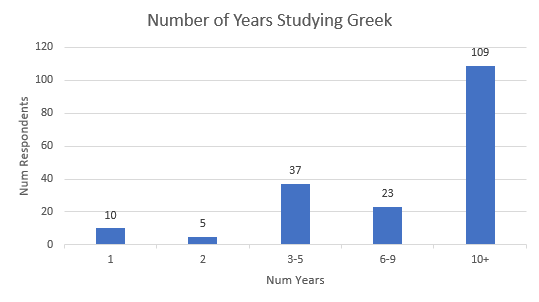
\includegraphics[width=.9\linewidth]{./images/years-studied.PNG}
\end{center}

\subsubsection{Satisfaction with current options}
\label{sec:org4277b2f}

\begin{center}
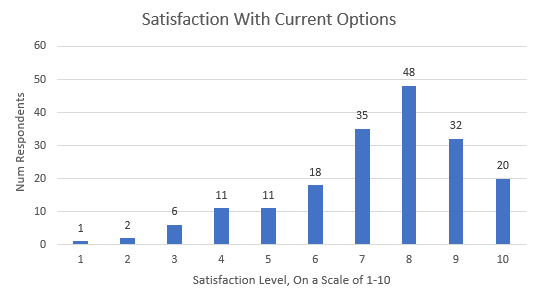
\includegraphics[width=.9\linewidth]{./images/satisfaction.PNG}
\end{center}

\subsubsection{Usage distribution of Greek entry methods}
\label{sec:orgf69b6d9}

\begin{center}
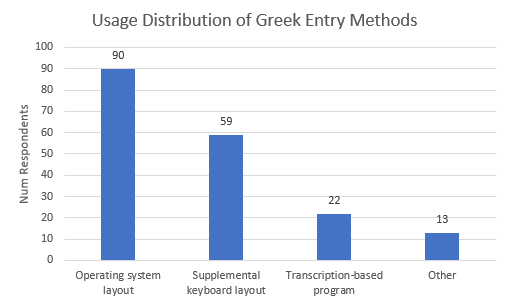
\includegraphics[width=.9\linewidth]{./images/entry-methods.PNG}
\end{center}

\subsubsection{Usage frequency of Greek entry methods}
\label{sec:orgaf6efcb}

\begin{center}
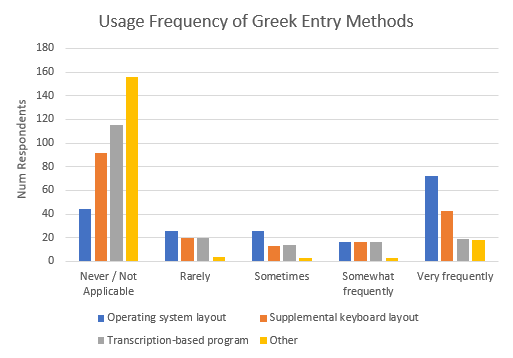
\includegraphics[width=.9\linewidth]{./images/entry-method-usage-distribution.PNG}
\end{center}

\subsubsection{Phonetic classification of primary entry method}
\label{sec:org3e69648}

\begin{center}
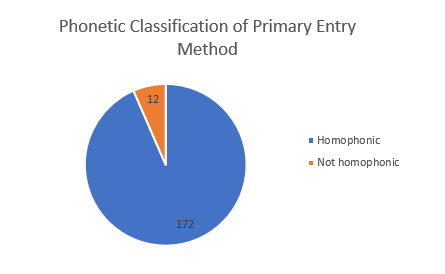
\includegraphics[width=.9\linewidth]{./images/homophonic.PNG}
\end{center}

\subsubsection{How often Greek is typed}
\label{sec:org1430f87}

\begin{center}
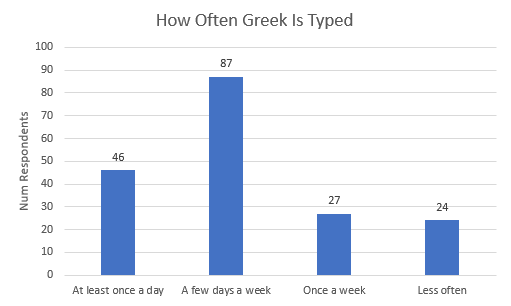
\includegraphics[width=.9\linewidth]{./images/typing-frequency.PNG}
\end{center}

\subsubsection{Typical quantity of Greek typed}
\label{sec:org48198ed}

\begin{center}
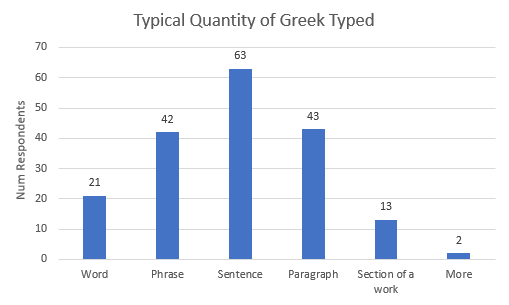
\includegraphics[width=.9\linewidth]{./images/typing-quantity.PNG}
\end{center}

\subsubsection{Preferences for entering diacritics}
\label{sec:org0220baa}

\begin{center}
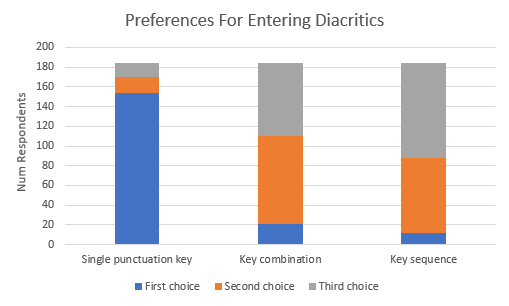
\includegraphics[width=.9\linewidth]{./images/diacritic-entry-preferences.PNG}
\end{center}

\subsubsection{Order preferences: handwriting}
\label{sec:org6aabf3c}

\begin{center}
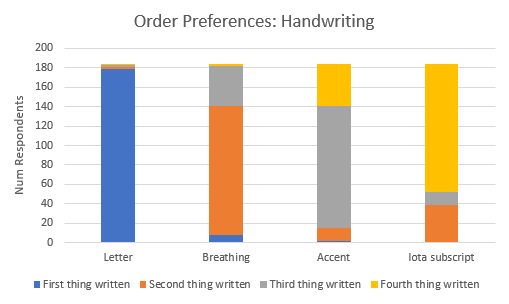
\includegraphics[width=.9\linewidth]{./images/diacritic-entry-order-writing.PNG}
\end{center}

\subsubsection{Order preferences: typing}
\label{sec:orgfc826aa}

\begin{center}
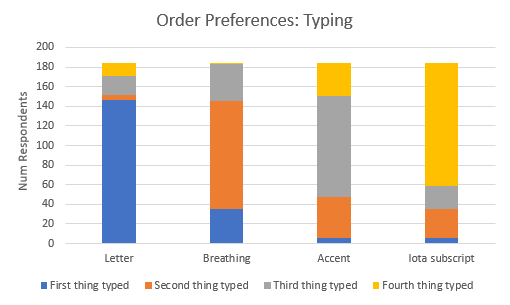
\includegraphics[width=.9\linewidth]{./images/diacritic-entry-order-typing.PNG}
\end{center}

\subsubsection{Ranking of possible features}
\label{sec:org4dca7a6}

\begin{center}
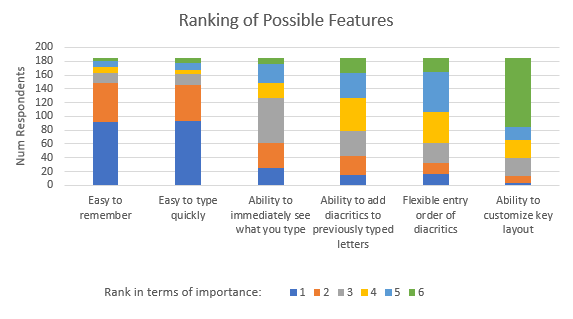
\includegraphics[width=.9\linewidth]{./images/ranking-of-possible-features.PNG}
\end{center}

\subsection{Greek layer}
\label{sec:org2f5c5dd}

\subsubsection{Complete layout graphic}
\label{sec:org744d84a}

\begin{center}
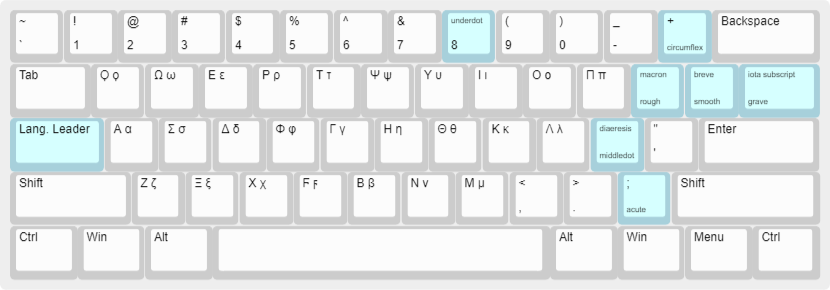
\includegraphics[width=.9\linewidth]{./images/greek-layer.png}
\end{center}

\subsubsection{Letter keymap}
\label{sec:org1c2ed23}

\begin{center}
\begin{tabular}{ll|ll}
Greek letter & Corresponding Key & Greek Letter & Corresponding Key\\
\hline
Α α & A a & Ν ν & N n\\
Β β & B b & Ξ ξ & X x\\
Γ γ & G g & Ο ο & O o\\
Δ δ & D d & Π π & P p\\
Ε ε & E e & Ρ ρ & R r\\
Ζ ζ & Z z & Σ σ & S s\\
Η η & H h & Τ τ & T t\\
Θ θ & J  j & Υ υ & U u\\
Ι ι & I i & Φ φ & F f\\
Κ κ & K k & Χ χ & C c\\
Λ λ & L l & Ψ ψ & Y y\\
Μ μ & M m & Ω ω & W w\\
\end{tabular}
\end{center}

\subsubsection{Diacritic/punctuation keymap}
\label{sec:org34fc2cb}

\begin{center}
\begin{tabular}{lll}
Grouping & Greek Character & Corresponding Key\\
\hline
Breathings & Rough & [\\
 & Smooth & ]\\
Accents & Acute & /\\
 & Grave & $\backslash$\\
 & Circumflex & =\\
Quantity & Iota Subscript & \(\vert{}\)\\
 & Macron & \{\\
 & Breve & \}\\
Punctuation & Greek Question Mark & ?\\
 & Greek Middle Dot & ;\\
Other & Diaeresis & :\\
 & Underdot & *\\
\end{tabular}
\end{center}

\subsection{Latin-script languages}
\label{sec:org805c871}

Out of the box, Latin, German, French, and Spanish should work. Other Latin-script languages that only use accents (e.g., Italian) will also work.

\subsubsection{Special characters}
\label{sec:org2050a9a}

\begin{center}
\begin{tabular}{lll}
Language & Character & Entry Sequence\\
\hline
French & ç & \{CapsLock\}c\\
 & Ç & \{CapsLock\}C\\
 & œ & \{CapsLock\}o\\
 & Π& \{CapsLock\}O\\
 & æ & \{CapsLock\}a\\
 & Æ & \{CapsLock\}A\\
German & ß & \{CapsLock\}s\\
 & ẞ & \{CapsLock\}S\\
Spanish & ñ & \{CapsLock\}n\\
 & Ñ & \{CapsLock\}N\\
 & ¿ & \{CapsLock\}?\\
 & ¡ & \{CapsLock\}!\\
\end{tabular}
\end{center}

\subsubsection{Diacritics}
\label{sec:orgd7c91be}

Note that the punctuation correspondences exactly mirror those of Greek where possible. This is to keep things consistent and reduce the total memory load.

\begin{center}
\begin{tabular}{lll}
Grouping & Diacritic & Entry Sequence\\
\hline
Accents & Acute & \{CapsLock\}/\\
 & Grave & \{CapsLock\}$\backslash$\\
 & Circumflex & \{CapsLock\}=\\
Quantity & Macron & \{CapsLock\}\{\\
 & Breve & \{CapsLock\}\}\\
Other & Diaeresis/umlaut & \{CapsLock\}:\\
\end{tabular}
\end{center}

\section{Works Cited}
\label{sec:orgcdf32a8}

\subsection{Proper citations}
\label{sec:orgbcd4cab}

\begin{hangparas}{.25in}{1}

Abandah, Gheith A., Tareq M. Malas, and Sinan Taifour. "Toward Optimal Arabic Keyboard Layout Using Genetic Algorithm." \textit{Proceedings of the 9th Int’l Middle Eastern Simulation Multiconference} (MESM 2008): 50-54. \\

Allen, W. Sidney. \textit{Vox Graeca: a Guide to the Pronunciation of Classical Greek}. Cambridge: Cambridge University Press, 1999. \\

Ansaldo, Ana Ines, and Ladan Ghazi-Saidi. "Second Language Word Learning through Repetition and Imitation: Functional Networks as a Function of Learning Phase and Language Distance." \textit{Frontiers in Human Neuroscience} 11 (2017): Paper No. 463. \\

Bannard, Colin and Danielle Matthews. "Stored Word Sequences in Language Learning The Effect of Familiarity on Children's Repetition of Four-Word Combinations." \textit{Psychological Science} 19 (2008): 241-248. \\

Choe, Pilsung, and Chen Liao. "Chinese Keyboard Layout Design Based on Polyphone Disambiguation and a Genetic Algorithm." \textit{International Journal of Human–Computer Interaction} 29:6 (2013): 391-403. \\

Chua, Shi Min, and Susan J. Rickard Liow. "The Locus of Word Frequency Effects in Skilled Spelling-to-Dictation." \textit{Quarterly Journal of Experimental Psychology} 67 (2014): 1720-1741. \\

Davis, Matt. "Cmabridge." cam.ac.uk. https:\textit{/www.mrc-cbu.cam.ac.uk/people/matt.davis/cmabridge} (accessed August 3, 2018). \\

Dhakal, Vivek, Anna Maria Feit, Per Ola Kristensson, and Antti Oulasvirta. "Observations on Typing from 136 Million Keystrokes." \textit{Proceedings of the 36th ACM Conference on Human Factors in Computing Systems} (CHI 2018): Paper No. 646. \\

Dunlosky, John, Elizabeth J. Marsh, Mitchell J. Nathan, Katherine A. Rawson, and Daniel T. Willingham. "Improving Students' Learning with Effective Learning Techniques: Promising Directions from Cognitive and Educational Psychology." \textit{Psychological Science in the Public Interest} 14 (2013): 4-58. \\

Feit, Anna Maria, Antti Oulasvirta, and Daryl Weir. "How We Type: Movement Strategies and Performance in Everyday Typing." \textit{Proceedings of the 2016 CHI Conference on Human Factors in Computing Systems} (CHI 2016): 4262-4273. \\

Kang, Sean H. K. "Spaced Repetition Promotes Efficient and Effective Learning: Policy Implications for Instruction." \textit{Policy Insights from the Behavioral and Brain Sciences} 3 (2016): 12-19. \\

Logan, Gordon D., and Motonori Yamaguchi. "Pushing Typists Back on the Learning Curve: Memory Chunking in the Hierarchical Control of Skilled Typewriting." \textit{Journal of Experimental Psychology: Learning, Memory, and Cognition} 42 (2016): 1919-1936. \\

Major, Wilfred E. "It’s Not the Size, It’s the Frequency: The Value of Using a Core Vocabulary in Beginning and Intermediate Greek." Winter 2008. \\

Nation, I. S. P. \textit{Learning Vocabulary in Another Language}. Cambridge: Cambridge University Press, 2001.

Norman, Donald, and David E. Rumelhart. "Simulating a Skilled Typist: A Study of Skilled Cognitive-Motor Performance." \textit{Cognitive Science} 6 (1982): 1-36. \\

Norvig, Peter. "English Letter Frequency Counts: Mayzner Revisited." Norvig.com. http:\textit{/www.norvig.com}mayzner.html (accessed August 3, 2018). \\

Piantadosi, Steven T. “Zipf’s Word Frequency Law in Natural Language: A Critical Review and Future Directions.” \textit{Psychonomic Bulletin & Review} 21.5 (2014): 1112-1130. \\

Raymond, Eric S. \textit{The Art of Unix Programming}. Boston: Addison-Wesley, 2004. \\

Saltzer, J. H., and Frans Kaashoek. \textit{Principles of Computer System Design: An Introduction}. Burlington, MA: Morgan Kaufmann, 2009. \\

Verbrugghe, Gerald P. "Transliteration or Transcription of Greek." \textit{The Classical World} 92, no. 6 (1999): 499-511. \\

\end{hangparas}

\subsection{Existing options for ancient Greek text entry}
\label{sec:orga7293a5}

\begin{center}
\begin{tabular}{ll}
GreekKeys & \url{https://classicalstudies.org/publications-and-research/about-greekkeys-2015}\\
SophoKeys & \url{http://benjaminblonder.org/sophokeys/}\\
Yudit & \url{http://yudit.org/}\\
da Grunk & \url{http://www.benwolkow.com/daGrunk/grunk-0.8.html\#daGrunk}\\
TypeGreek.com & \url{http://www.typegreek.com/}\\
Antioch & \url{http://www.users.dircon.co.uk/\~hancock/antioch.htm}\\
\end{tabular}
\end{center}
\end{document}
